\section{Projeto de controladores no \texorpdfstring{plano $ z $}{plano-z}}

\begin{frame}{Introdução}
\begin{block}{Contextualização}
	\begin{itemize}
		\item A principal dificuldade dos projetos no plano $ z $ é a escolha dos polos de malha fechada para que resultem transientes aceitáveis com razoável robustez frente às variações da planta.
		\item \textbf{Os polos do plano $ \bm{z} $ podem ser obtidos por meio do mapeamento dos polos em $ \bm{s} $}.	Dado um desejado amortecimento para um par de polos, no plano $ s $ os polos estão sobre retas bem conhecidas enquanto em $ z $ estão sobre um \textbf{“amontoado de curvas”}. Portanto, a sensibilidade do sobressinal com relação à variação de parâmetros é muito grande.
	\end{itemize}
\end{block}
\end{frame}

\begin{frame}{Requisitos de desempenho no plano $z$}
\begin{block}{Contextualização}
	\begin{itemize}
		\item A figura abaixo é um mapa do disco unitário no plano $z$ no qual são sobrepostas respostas de tempo discretas do sistema que correspondem a várias localizações típicas dos polos do plano $z$.
		\item Elas podem ser usadas para traduzir as especificações de desempenho de resposta dinâmica em uma região de polos aceitáveis.
	\end{itemize}
\end{block}
\centerline{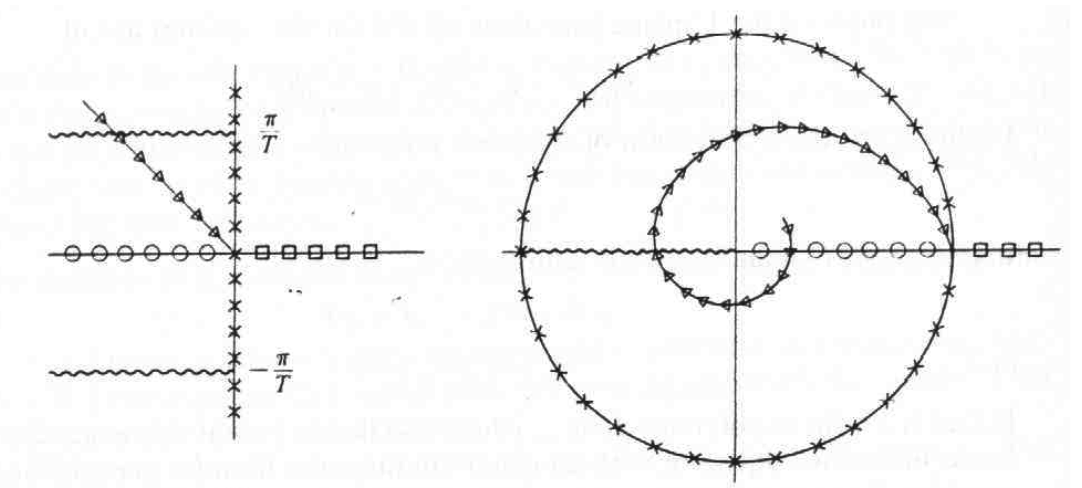
\includegraphics[width=0.8\linewidth]{Figuras/Ch11/fig1.PNG}}
\end{frame}

\begin{frame}{Requisitos de desempenho no plano $z$}
\begin{block}{Contextualização}
	\begin{itemize}
		\item Sabendo que
	\end{itemize}
$$s = -\zeta \omega_n + j \omega_d,$$
	\begin{itemize}
		\item[] temos
	\end{itemize}
$$z = r\text{e}^{j\theta}, \quad \text{onde} \quad r = \text{e}^{-\zeta \omega_n T} \quad \text{e} \quad \theta = \omega_d T$$
\vspace{-0.3cm}
	\begin{itemize}
		\item A frequência natural em $s$ mapeia o \textbf{ângulo do polo} em coordenadas polares no plano $z$, já que $\theta = \omega_d T$ onde $\omega_d = \omega_n \sqrt{1 - \zeta^2}$.
		\item O tempo de acomodação é inversamente proporcional à magnitude da parte real de um polo no plano $s$ ($\sigma = \zeta \omega_n$), que mapeia o \textbf{raio do polo} no plano $z$, já que $r = \text{e}^{-\zeta \omega_n T}$.
		\item O \textit{overshoot} varia inversamente com o coeficiente de amortecimento. Deste modo, linhas de amortecimento constante no plano $s$ são mapeadas em \textbf{espirais logarítmicos} no plano $z$.
	\end{itemize}
\end{block}
\end{frame}

\begin{frame}{Requisitos de desempenho no plano $z$}
\centerline{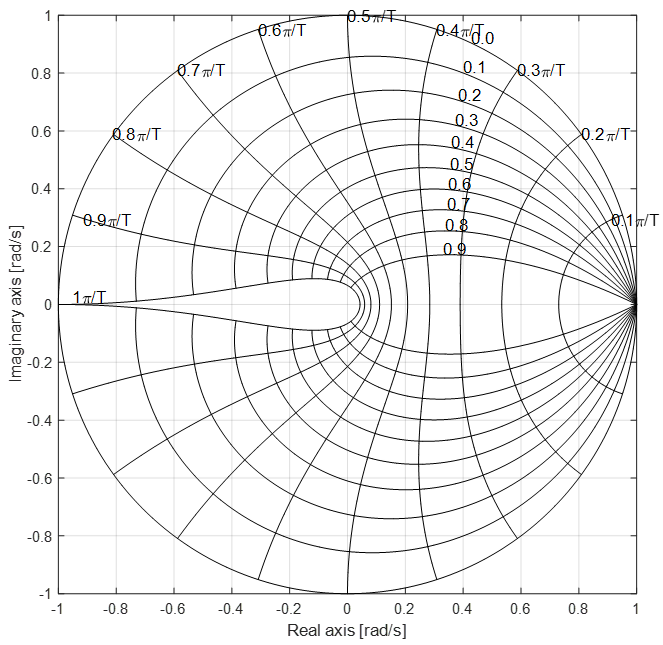
\includegraphics[width=0.65\linewidth]{Figuras/Ch11/fig2.png}}
\end{frame}

\begin{frame}{Requisitos de desempenho no plano $z$}
\begin{block}{Contornos de frequência constante}
	\begin{itemize}
		\item As linhas destacadas na figura abaixo são as linhas de frequência constante, expressas na forma $\alpha \pi/T, \  \text{onde} \ 0 \leq \alpha \leq 1$.
	\end{itemize}
\end{block}
\centerline{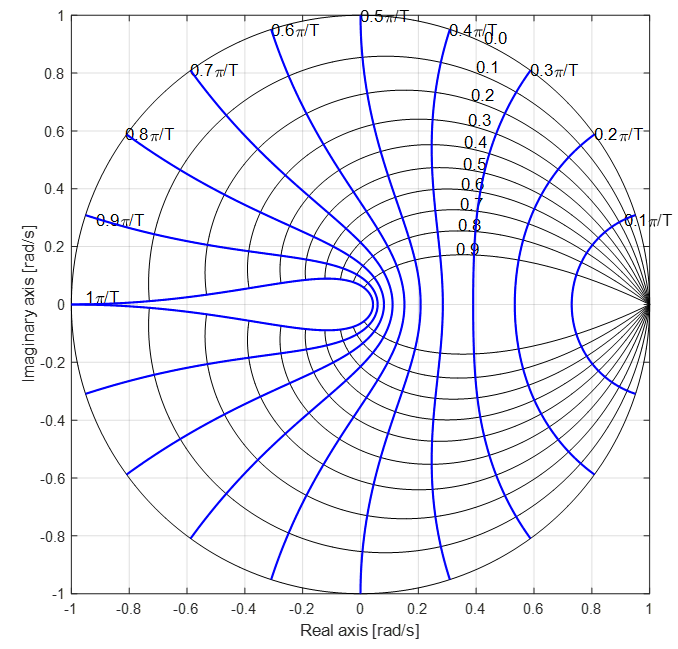
\includegraphics[width=0.5\linewidth]{Figuras/Ch11/fig3.png}}
\end{frame}

\begin{frame}{Requisitos de desempenho no plano $z$}
\begin{block}{Contornos de frequência constante - Exemplo}
	\begin{itemize}
		\item Considerando $\omega_n = \num{31,34}$ rad/s e $T = \num{0,1}$ s, podemos escrever  $\omega_n = (\omega_nT/\pi) \cdot (\pi/T)$.
	\end{itemize}
\end{block}
\centerline{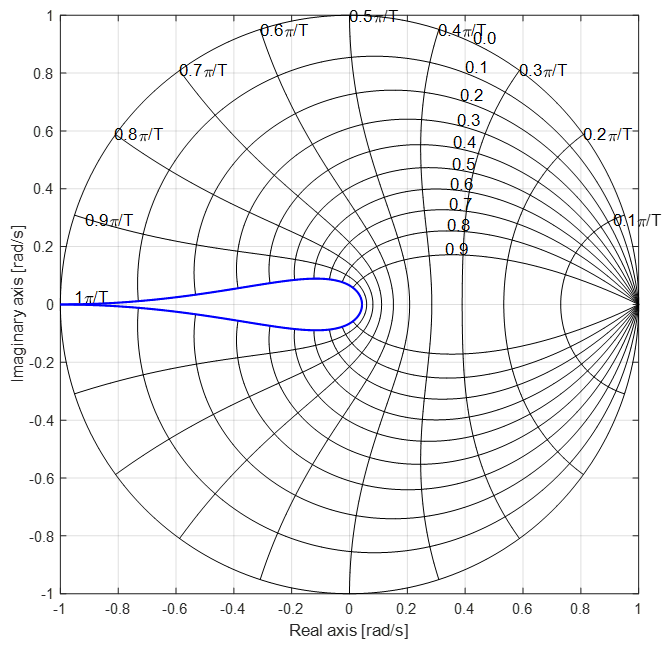
\includegraphics[width=0.5\linewidth]{Figuras/Ch11/fig4.png}}
\end{frame}

\begin{frame}{Requisitos de desempenho no plano $z$}
\begin{block}{Contornos de coeficiente de amortecimento constante}
	\begin{itemize}
		\item Locais mais próximos dos contornos internos no plano $z$ ou mais longe do plano $s$ correspondem a um fator de amortecimento mais alto.
	\end{itemize}
\end{block}
\centerline{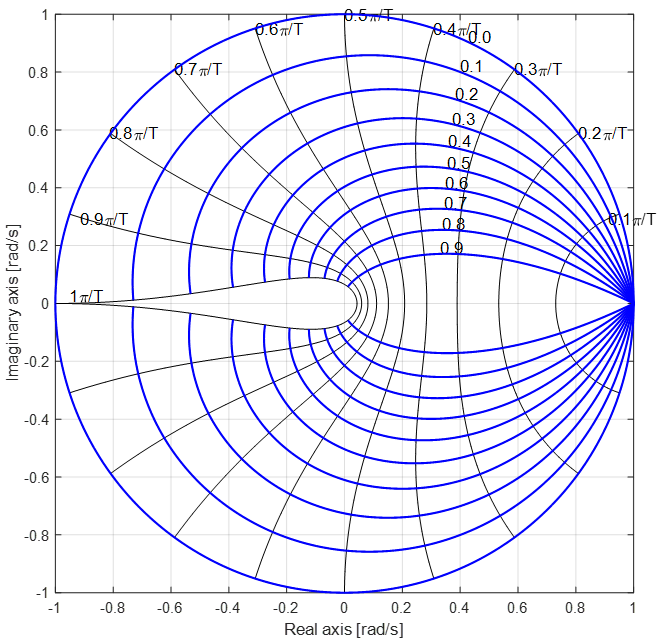
\includegraphics[width=0.5\linewidth]{Figuras/Ch11/fig5.png}}
\end{frame}

\begin{frame}{Requisitos de desempenho no plano $z$ - Exemplo \#01}
\begin{block}{Problema}
Considere uma função de transferência contínua de segunda ordem com frequência natural de $\num{12,7}$ rad/s e coeficiente de amortecimento de $\num{0,1}$. Encontre o equivalente discreto e a sua região no plano $z$.
\end{block}
\end{frame}

\begin{frame}{Requisitos de desempenho no plano $z$ - Exemplo \#01}
\begin{block}{Resolução}
\begin{itemize}
    \item A função de transferência contínua pode ser escrita como sendo:
\end{itemize}
$$G(s) = \dfrac{\omega_n^2}{s^2+ 2\zeta \omega_n s +\omega_n^2} = \dfrac{\num{161,3}}{s^2 + \num{2,54}s + \num{161,3}}$$
\begin{itemize}
    \item Utilizando ZOH (considerando $T = \num{0,1}$ s), obtemos:
\end{itemize}
$$G(z) = \dfrac{\num{0,649}z + \num{0,593}}{z^2- \num{0,532}z + \num{0,775}}$$
\begin{itemize}
    \item O raio do polo no plano $z$ é dado por:
\end{itemize}
$$z = \text{e}^{-\zeta \omega_n T} = \num{0,8807}$$
\begin{itemize}
    \item De fato, os polos em $z$ estão localizados em $z_{1,2} = \num{0,266} \pm j\num{0,839}$, o que corresponde a um módulo (raio) de $\num{0,8807}$.
\end{itemize}
\end{block}
\end{frame}

\begin{frame}{Requisitos de desempenho no plano $z$ - Exemplo \#01}
\begin{block}{Resolução}
\begin{itemize}
    \item A frequência natural de $\num{12,7}$ rad/s corresponde à linha de contorno $\num{0,4}\pi/T$. \textbf{Os dois polos estão localizados nas interseções dos dois contornos.}
\end{itemize}
\end{block}
\centerline{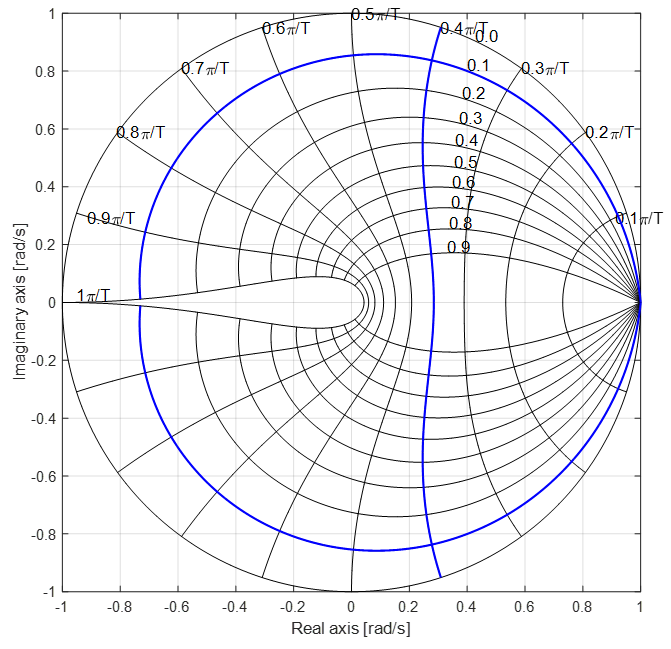
\includegraphics[width=0.48\linewidth]{Figuras/Ch11/fig6.png}}
\end{frame}

\begin{frame}{Projeto no plano $z$}
\begin{block}{Considerações}
\begin{itemize}
    \item Este método de projeto determina o controlador discreto \textbf{diretamente} no plano $ z $, diferentemente da emulação. Com isso, está sendo \textbf{eliminada a natureza de aproximações do projeto}.
    \item A implementação do controlador discreto se dá por meio de uma \textbf{equação de diferenças}, assim como na emulação.
    \item O controlador discreto pode ser simulado e testado na malha de controle digital (a \textbf{discretização da planta via ZOH} torna-se obrigatória independente da simulação, já que o controlador é projetado no plano $z$) para a verificação dos requisitos de desempenho.
    \item Existem duas técnicas para projetar um controlador digital no plano $z$, assim como na emulação:
    \begin{enumerate}
        \item Projeto pelo lugar das raízes;
        \item Projeto pela imposição algébrica de polos.
    \end{enumerate}
\end{itemize}
\end{block}
\end{frame}

\begin{frame}{Projeto pelo lugar das raízes - Exemplo \#01}
\begin{block}{Problema}
	Implementar um controlador discreto no plano $z$, utilizando o lugar das raízes, para a planta
	$$ G_p(s)=\dfrac{1}{s(s+1)}, $$
	de modo que $ M_p=\num{16,3}\% $ e $ T_p=\; $\SI{1}{\second}, quando um degrau for aplicado na entrada.
\end{block}
\end{frame}

\begin{frame}{Projeto pelo lugar das raízes - Exemplo \#01}
\begin{block}{Resolução}
\begin{itemize}
    \item Utilizando as métricas de desempenho que foram dadas:
\end{itemize}
	\begin{align*}
		M_p&=\exp{\left( \dfrac{-\pi\zeta}{\sqrt{1-\zeta^{2}}}\right) }\rightarrow \ln\num{0,163}=\dfrac{-\pi\zeta}{\sqrt{1-\zeta^{2}}}\rightarrow\zeta\approx\num{0,5}\\
		T_p&=\dfrac{\pi}{\omega_d}\therefore 1=\dfrac{\pi}{\omega_d}\rightarrow\omega_d=\pi\;\si{\radian\per\second}\therefore\omega_n=\SI{3,628}{\radian\per\second}
	\end{align*}
\begin{itemize}
    \item Com isso, os polos complexos dominantes devem estar localizados em:
\end{itemize}
	
	\[ s_{1,2}=-\zeta\omega_n\pm j\omega_d\Rightarrow s_{1,2}=-\num{1,81}\pm j\pi \]

\begin{itemize}
    \item A resposta transitória apresenta oscilações com período:
\end{itemize}

	\[ T_d=\dfrac{2\pi}{\omega_d}=\dfrac{2\pi}{\pi}=\SI{2}{\second} \]
\end{block}
\end{frame}

\begin{frame}{Projeto pelo lugar das raízes - Exemplo \#01}
\begin{block}{Resolução}
\begin{itemize}
    \item Escolhe-se um período de amostragem pelo menos $ 10\times $ menor. Logo,
\end{itemize}
	 
	\[ T=\SI{0,2}{\second} \]

\begin{itemize}
    \item No plano $z$, os polos são mapeados em:
\end{itemize}
\begin{align*}
		z_{1,2}=\text{e}^{-\num{1,81}T\pm\pi jT}\text{, com } T=\SI{0,2}{\second}\therefore
		z_{1,2}&=\text{e}^{-\num{1,81}\cdot\num{0,2}}\cdot\text{e}^{\num{0,2}\pi j}\\
		&=\num{0,6957}\left[ \cos{(\num{0,2}\tikzmark{p1}\pi)}\pm\sen{(\num{0,2}\tikzmark{p2}\pi)}\right]\\
		&=\num{0,6957}\left( \num{0,8090}\pm j\num{0,5877} \right)\\
		&=\num{0,5629}\pm\num{0,4090}j
		\end{align*}
\end{block}
    \begin{tikzpicture}[overlay, remember picture]
	\draw[->] (p1)+(0,0.25) -- +(0.5,0.5) node[above right=0pt, yshift=-3pt,name=p3] {\si{\radian}};
	\draw[->] (p2)+(-0.2,0.25) -- (p3);
	\end{tikzpicture}
\end{frame}


\begin{frame}{Projeto pelo lugar das raízes - Exemplo \#01}
\begin{block}{Resolução}
\begin{itemize}
    \item Como o controlador será projetado diretamente no plano $z$, o próximo passo é discretizar a planta via ZOH.
\end{itemize}
	Função de transferência $ G_p(z) $ do subsistema D/A + planta + A/D:
	
	\begin{align*}
		\dfrac{G_p(s)}{s}=\dfrac{1}{s^{2}(s+1)}=\dfrac{A}{s}+\dfrac{B}{s^{2}}+\dfrac{C}{s+1}\Rightarrow &1=As(s+1)+B(s+1)+Cs^{2}\\
		&1=(A+C)s^{2}+(A+B)s+B
	\end{align*}
	\[\makebox[13.5em]{}\left\lbrace\begin{aligned}
	B&=1 \\
	A+B&=0\rightarrow A=-1\\
	A+C&=0 \rightarrow C=1
	\end{aligned}\right. \]
\end{block}
\end{frame}


\begin{frame}{Projeto pelo lugar das raízes - Exemplo \#01}
\begin{block}{Resolução}
	\begin{align*}
	G_p(z)&=\frac{z-1}{z}\left[ \mathcal{Z}\left\lbrace  -1+kT+\text{e}^{-1kT}\right\rbrace   \right]=\\
	&= \frac{\cancel{z-1}}{\cancel{z}}\left[ \frac{\cancel{-z}}{\cancel{z-1}}+\frac{\num{0,2}\cancel{z}}{(z-1)^{\cancel{2}}}+\frac{\cancel{z}}{z-\text{e}^{-1\cdot T}}\right]=\\
	&=-1+\frac{\num{0,2}}{z-1}+\frac{z-1}{z-\num{0,8187}}=\\
	&=\frac{-(z-1)(z-\num{0,8187})+\num{0,2}(z-\num{0,8187})+(z-1)^{2}}{(z-1)(z-\num{0,8187})}=\\
	&=\frac{\cancel{-z^{2}}+\num{1,8187}z-\num{0,8187}+\num{0,2}z-\num{0,1637}\cancel{+z^{2}}-2z+1}{(z-1)(z-\num{0,8187})}=\\
	&=\frac{\num{0,0187}(z+\num{0,9355})}{(z-1)(z-\num{0,8187})}
	\end{align*}
\end{block}
\end{frame}


\begin{frame}{Projeto pelo lugar das raízes - Exemplo \#01}
\begin{block}{Resolução}
\begin{itemize}
    \item Deve-se encontrar uma função de transferência $ G_c(z) $ de modo que o \textbf{lugar das raízes passe pelos polos de malha fechada desejados. A diferença é que agora estamos limitados ao interior do círculo de raio unitário}.
\end{itemize}
	
	\[ G_c(z)=\dfrac{K(z+C_1)}{(z+C_2)} \]
	
\begin{itemize}
    \item O sistema em malha aberta (considerando o controlador discreto e a planta discreta) é:
\end{itemize}

	\[ \text{sysMA}=\frac{K(z+C_1)}{(z+C_2)}\cdot\frac{\num{0,0187}(z+\num{0,9355})}{(z-1)(z-\num{0,8187})} \]
\end{block}
\end{frame}

\begin{frame}{Projeto pelo lugar das raízes - Exemplo \#01}
\centerline{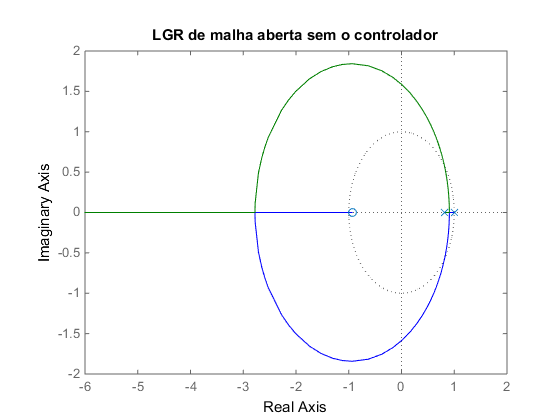
\includegraphics[width=0.8\linewidth]{Figuras/Ch11/fig7.png}}
\end{frame}


\begin{frame}{Projeto pelo lugar das raízes - Exemplo \#01}
\begin{block}{Resolução}
\begin{itemize}
    \item Uma possível solução para encontrar $C_1$ é cancelar o polo estável do sistema em malha aberta com o zero do controlador. Sendo assim, cancelando o polo estável ($ z-\num{0,8187} $) do sistema em malha aberta, tem-se que $ C_1=-\num{0,8187} $. Logo,
\end{itemize}
\[ \text{sysMA}=\dfrac{\num{0,0187}K(z+\num{0,9355})}{(z+C_2)(z-1)} \]
\end{block}
\end{frame}


\begin{frame}{Projeto pelo lugar das raízes - Exemplo \#01}
\begin{block}{Resolução}
\begin{itemize}
    \item Calcula-se $ C_2 $ pela condição de fase:
\end{itemize}
	
	\[ \left. \left( \underbrace{\strut\phase{z+\num{0,9355}}}_{(\ang{15,26})}-\underbrace{\strut\phase{z+C_2}}_{\tg^{-1}\left( \frac{\num{0,4090}}{\num{0,5629}+C_2}\right)}-\underbrace{\strut\phase{z-1}}_{(-\ang{43,09})}\right) \right|_{z=\num{0,5629}+\num{0,4090}j}=\ang{-180} \]
	
	\begin{align*}
	\ang{-238,35}&=-\tg^{-1}\left( \frac{\num{0,4090}}{\num{0,5629}+C_2}\right)& &\\
	\cancel{-}\num{1,622}&=\cancel{-}\frac{\num{0,4090}}{\num{0,5629}+C_2}&\Rightarrow\num{0,913}+\num{1,622}C_2&=\num{0,4090}\\
	& & \num{1,622}C_2&=-\num{0,504}\\
	& & C_2&= -\num{0,3109}
	\end{align*}
\end{block}
\end{frame}


\begin{frame}{Projeto pelo lugar das raízes - Exemplo \#01}
\begin{block}{Resolução}
\begin{itemize}
    \item Calcula-se $ K $ pela condição de módulo:
\end{itemize}
	\[ \eval{\left| \frac{\num{0,0187}K(z+\num{0,9355})}{(z-\num{0,3109})(z-1)} \right| }_{z=\num{0,5629}+\num{0,4090}j}=1\Rightarrow K=\num{9,9} \]
\begin{itemize}
    \item Com isso, o \textbf{controlador discreto} é dado por:
\end{itemize}
	\[ G_c(z)=\dfrac{\num{9,9}(z-\num{0,8187})}{(z-\num{0,3109})} \]
\end{block}
\end{frame}

\begin{frame}{Projeto pelo lugar das raízes - Exemplo \#01}
\centerline{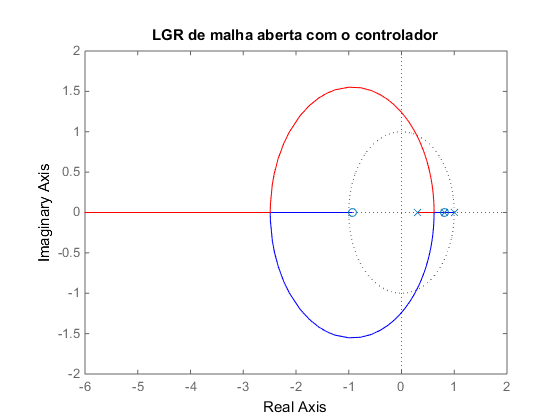
\includegraphics[width=0.8\linewidth]{Figuras/Ch11/fig8.png}}
\end{frame}

\begin{frame}{Projeto pelo lugar das raízes - Exemplo \#01}
\begin{block}{Resolução}
$$\dfrac{U(z)}{E(z)}=\dfrac{\num{9,9}(z-\num{0,8187})}{z-\num{0,3109}}$$

$$u[k+1] - \num{0,3109} u[k]=\num{9,9}e[k+1]-\num{8,1051}e[k]$$

Aplicando um atraso, temos:\\
$$u[k]=\num{0,3109}u[k-1]+\num{9,9}e[k]-\num{8,1051}e[k-1]$$
\end{block}
\end{frame}

\begin{frame}{Projeto pelo lugar das raízes - Exemplo \#01}
\begin{block}{Resolução}
\begin{itemize}
    \item A \textbf{função de transferência em malha fechada} é, portanto,
\end{itemize}
$$\dfrac{Y(z)}{R(z)}=\dfrac{G_c(z)G_p(z)}{1+G_c(z)G_p(z)}=\dfrac{\num{0,1851}z+\num{0,1731}}{z^{2}-\num{1,1258}z+\num{0,4841}}$$

$$y[k]=\num{1,1258}y[k-1]-\num{0,4841}y[k-2]+\num{0,1851}r[k-1]+\num{0,1731}r[k-2]$$
\end{block}
\end{frame}

\begin{frame}{Projeto pelo lugar das raízes - Exemplo \#01}
\centerline{
\includegraphics[width=0.8\linewidth]{Figuras/Ch11/fig9.png}}
\end{frame}


\begin{frame}{Projeto pela imposição algébrica de polos - Exemplo \#01}
\begin{block}{Problema}
	Implementar um controlador discreto no plano $z$, utilizando o lugar das raízes, para a planta
	$$ G_p(s)=\dfrac{1}{s(s+1)}, $$
	de modo que $ M_p=16,3\% $ e $ T_p=\; $\SI{1}{\second}, quando um degrau for aplicado na entrada.
\end{block}
\end{frame}

\begin{frame}{Projeto pela imposição algébrica de polos - Exemplo \#01}
\begin{block}{Resolução}
\begin{itemize}
    \item Nesta técnica \textbf{os polos do controlador são alocados} na posição que atenda às especificações do projeto.
\end{itemize}
	\[ \left. \begin{aligned}
	G_p(z)&=\frac{\num{0,0187}(z+\num{0,9355})}{(z-1)(z-\num{0,8187})}
	\end{aligned}\right\rbrace \text{grau $ n=2 $} \]
\centering
O controlador deve ter grau $ m\geqslant n-1 $.
\vspace{0.4cm}
\begin{itemize}
    \item Assume-se $ m=1 $, logo
\end{itemize}
\[ G_c(z)=K\dfrac{(z+C_1)}{(z+C_2)} \]
\end{block}
\end{frame}

\begin{frame}{Projeto pela imposição algébrica de polos - Exemplo \#01}
\begin{block}{Resolução}
\begin{itemize}
    \item O sistema em malha aberta (considerando o controlador discreto e a planta discreta) é:
\end{itemize}

	\[ \text{sysMA}=\frac{K(z+C_1)}{(z+C_2)}\cdot\frac{\num{0,0187}(z+\num{0,9355})}{(z-1)(z-\num{0,8187})} \]
\end{block}
\end{frame}

\begin{frame}{Projeto pela imposição algébrica de polos - Exemplo \#01}
\centerline{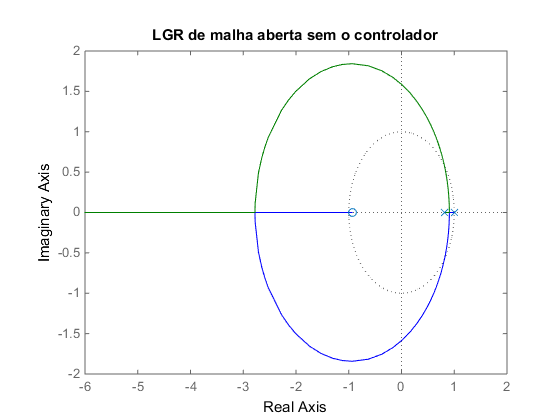
\includegraphics[width=0.8\linewidth]{Figuras/Ch11/fig10.png}}
\end{frame}

\begin{frame}{Projeto pela imposição algébrica de polos - Exemplo \#01}
	\begin{block}{Resolução}
\begin{itemize}
    \item Uma possível solução para encontrar $C_1$ é cancelar o polo estável do sistema em malha aberta com o zero do controlador. Sendo assim, cancelando o polo estável ($ z-\num{0,8187} $) do sistema em malha aberta, tem-se que $ C_1=-\num{0,8187} $. Logo,
\end{itemize}
	\[ \text{sysMA}=\frac{\num{0,0187}K(z+\num{0,9355})}{(z+C_2)(z-1)} \]
\begin{itemize}
\vspace{-0.2cm}
    \item A \textbf{função de transferência de malha fechada} é dada por:
\end{itemize}		
		\[ \text{sysMF}=\frac{\num{0,0187}K(z+\num{0,9355})}{(z+C_2)(z-1)+\num{0,0187}K(z+\num{0,9355})} \]
\begin{itemize}
\vspace{-0.2cm}
    \item Deste modo, a equação característica pode ser expressa como sendo:
\end{itemize}
\[  D(z)=z^{2}+(\num{0,0187}K+C_2-1)z+\num{0,0175}K-C_2 \]
	\end{block}
\end{frame}

\begin{frame}{Projeto pela imposição algébrica de polos - Exemplo \#01}
	\begin{block}{Resolução}
\begin{itemize}
    \item Considerando os polos desejados (\textit{vide exemplo anterior}), temos que a equação característica é dada por:
\end{itemize}
		\begin{align*}
			D(z)&=(z-\num{0,5629}-\num{0,4090}j)(z-\num{0,5629}+\num{0,4090}j)\\
		    D(z)&=z^{2}-\num{1,1258}z+\num{0,4841}
		\end{align*}
		\vspace{-0.3cm}
\begin{itemize}
    \item Comparando as duas equações características, obtém-se:
\end{itemize}		
		\begin{gather*}
			K=\num{9,9}\\
			C_2=-\num{0,3109}
		\end{gather*}
		\vspace{-0.3cm}
\begin{itemize}
    \item Com isso, o \textbf{controlador discreto} é dado por:
\end{itemize}
		\[ G_c(z)=\dfrac{\num{9,9}(z-\num{0,8187})}{(z-\num{0,3109})} \]
\end{block}
\end{frame}

\begin{frame}{Projeto pela imposição algébrica de polos - Exemplo \#01}
\centerline{
\includegraphics[width=0.8\linewidth]{Figuras/Ch11/fig11.png}}
\end{frame}

\begin{frame}{Projeto pela imposição algébrica de polos - Exemplo \#01}
\begin{block}{Resolução}
$$\dfrac{U(z)}{E(z)}=\dfrac{\num{9,9}(z-\num{0,8187})}{z-\num{0,3109}}$$

$$u[k+1] - \num{0,3109} u[k]=\num{9,9}e[k+1]-\num{8,1051}e[k]$$

Aplicando um atraso, temos:\\
$$u[k]=\num{0,3109}u[k-1]+\num{9,9}e[k]-\num{8,1051}e[k-1]$$
\end{block}
\end{frame}

\begin{frame}{Projeto pela imposição algébrica de polos - Exemplo \#01}
\begin{block}{Resolução}
\begin{itemize}
    \item A \textbf{função de transferência em malha fechada} é, portanto,
\end{itemize}
$$\dfrac{Y(z)}{R(z)}=\dfrac{G_c(z)G_p(z)}{1+G_c(z)G_p(z)}=\dfrac{\num{0,1851}z+\num{0,1731}}{z^{2}-\num{1,1258}z+\num{0,4841}}$$

$$y[k]=\num{1,1258}y[k-1]-\num{0,4841}y[k-2]+\num{0,1851}r[k-1]+\num{0,1731}r[k-2]$$
\end{block}
\end{frame}

\begin{frame}{Projeto pela imposição algébrica de polos - Exemplo \#01}
\centerline{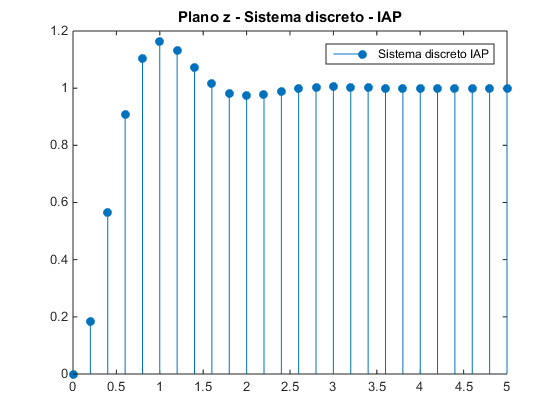
\includegraphics[width=0.8\linewidth]{Figuras/Ch11/fig12.png}}
\end{frame}

\begin{frame}{Comparação entre os métodos}
\centerline{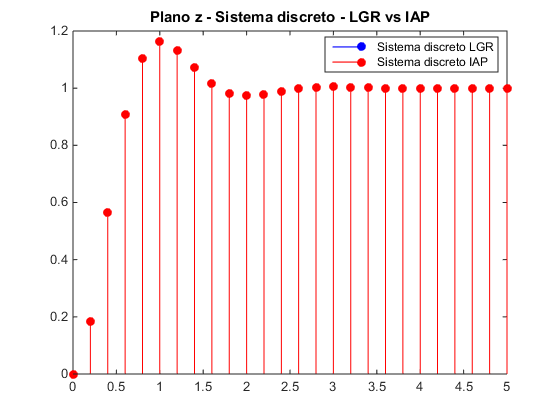
\includegraphics[width=0.8\linewidth]{Figuras/Ch11/fig13.png}}
\end{frame}

\begin{frame}{Comparação entre os métodos (emulação vs plano $z$)}
\centerline{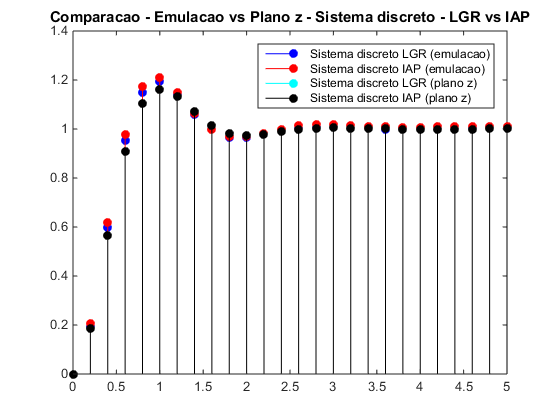
\includegraphics[width=0.8\linewidth]{Figuras/Ch11/fig14.png}}
\end{frame}

\frame{
\frametitle{Exercícios}
\begin{block}{}
01. Considere o diagrama de blocos de um sistema em malha fechada.
\begin{enumerate}
    \item[(a)] Projete um controlador digital, diretamente no plano $z$, utilizando a técnica do lugar das raízes, sabendo que é desejado que os polos dominantes tenham um fator de amortecimento de $\num{0,5}$ e um tempo de acomodação de $2$ s para uma entrada em degrau. Assuma T = $T_d/9$ s. Determine ainda o erro em regime permanente para uma entrada $r(t) = e^2  t$, para todo $t \geq 0$, onde $e$ é uma constante matemática, conhecida como o número de Euler.
    \item[(b)] Repita considerando a técnica da imposição algébrica de polos.
    \item[(c)] Simule e compare os resultados pelo \MATLAB.
    \item[(d)] Compare estes dois resultados com os do capítulo anterior (emulação).
\end{enumerate}
\end{block}
\centerline{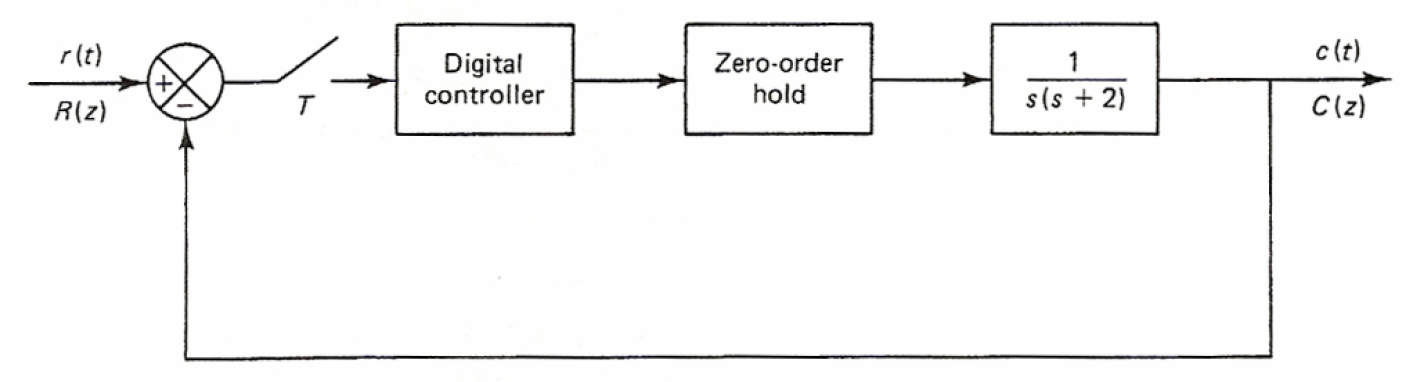
\includegraphics[width=0.68\linewidth]{Figuras/Ch10/fig9.PNG}}
}

\frame{
\frametitle{Referências e exercícios complementares}
\begin{itemize}
\item FRANKLIN, Gene F.; POWELL, J. David; WOLKMAN, Michael L. Digital Control of Dynamic Systems, 3 ed. Addison-Wesley, 1998.
\end{itemize}
\centering{\alert{Página 270 - \textbf{Capítulo 7}}}
}